% Numerical Integration: Trapezoidal and Simpson Rules
% The properly typeset version of the badly formatted Word document (word-before.docx).
\documentclass[11pt,a4paper]{article}

\usepackage[T1]{fontenc}
\usepackage[utf8]{inputenc}
\usepackage[a4paper,margin=2.7cm]{geometry}
\usepackage{libertinus}
\usepackage{microtype}
\usepackage{amsmath,amssymb,amsthm,mathtools}
\usepackage{booktabs,siunitx}
\usepackage{tikz,pgfplots}
\pgfplotsset{compat=1.18}
\usepackage{caption}
\captionsetup{font=small,labelfont=bf,format=hang}
\usepackage[colorlinks=true,linkcolor=blue!55!black,citecolor=blue!55!black,urlcolor=blue!55!black]{hyperref}
\usepackage[capitalise]{cleveref}
\usepackage[backend=biber,style=numeric,sorting=none]{biblatex}
\addbibresource{references.bib}

\newtheorem{proposition}{Proposition}
\DeclareMathOperator{\erf}{erf}
\sisetup{output-exponent-marker=\ensuremath{\mathrm{e}}}

\title{\bfseries Numerical Integration:\\ Trapezoidal and Simpson Rules}
\author{N'sol\'e Samson Yamontche\\[2pt]\small UNSTIM, Benin}
\date{12 October 2026}

\begin{document}
\maketitle

\begin{abstract}
\noindent
This note presents two simple methods for computing definite integrals numerically: the trapezoidal rule and Simpson's rule.
We state their error bounds, test both rules on a single example, and compare the observed errors with the theoretical rates.
\end{abstract}

\section{Introduction}
Many integrals cannot be expressed with elementary functions. For example, the integral of $e^{-x^{2}}$ over $[0,1]$ has no closed form in elementary terms, so numerical methods are needed.
Given a function $f$ on an interval $[a,b]$, we want to approximate
\begin{equation}
  I = \int_a^b f(x)\,\mathrm{d}x.
  \label{eq:integral}
\end{equation}

\section{The trapezoidal rule}
Divide $[a,b]$ into $n$ equal subintervals of width $h=(b-a)/n$, with nodes $x_i=a+ih$. The \emph{trapezoidal rule} is
\begin{equation}
  T_n = h\left[\frac{f(a)}{2} + \sum_{i=1}^{n-1} f(x_i) + \frac{f(b)}{2}\right].
  \label{eq:trap}
\end{equation}

\begin{proposition}[Error of the trapezoidal rule]\label{prop:trap}
If $f\in C^{2}[a,b]$, then
\begin{equation}
  \lvert I - T_n\rvert \le \frac{(b-a)\,h^{2}}{12}\,\max_{x\in[a,b]}\lvert f''(x)\rvert .
  \label{eq:trap-err}
\end{equation}
\end{proposition}

\section{Simpson's rule}
If $n$ is even, \emph{Simpson's rule} is
\begin{equation}
  S_n = \frac{h}{3}\Bigl[f(x_0) + 4\!\!\sum_{\substack{i=1\\ i\ \text{odd}}}^{n-1}\!\! f(x_i)
        + 2\!\!\sum_{\substack{i=2\\ i\ \text{even}}}^{n-2}\!\! f(x_i) + f(x_n)\Bigr].
  \label{eq:simpson}
\end{equation}

\begin{proposition}[Error of Simpson's rule]\label{prop:simpson}
If $f\in C^{4}[a,b]$, then
\begin{equation}
  \lvert I - S_n\rvert \le \frac{(b-a)\,h^{4}}{180}\,\max_{x\in[a,b]}\lvert f^{(4)}(x)\rvert .
  \label{eq:simpson-err}
\end{equation}
\end{proposition}

\section{Numerical experiment}
We take $f(x)=e^{-x^{2}}$ on $[0,1]$. The exact value is
$I=\tfrac{\sqrt{\pi}}{2}\erf(1)\approx 0.7468241328$.
\Cref{fig:trap} shows the function and the four trapezoids used for $n=4$, and \cref{tab:results} lists the approximations and their errors.

\begin{figure}[htbp]
  \centering
  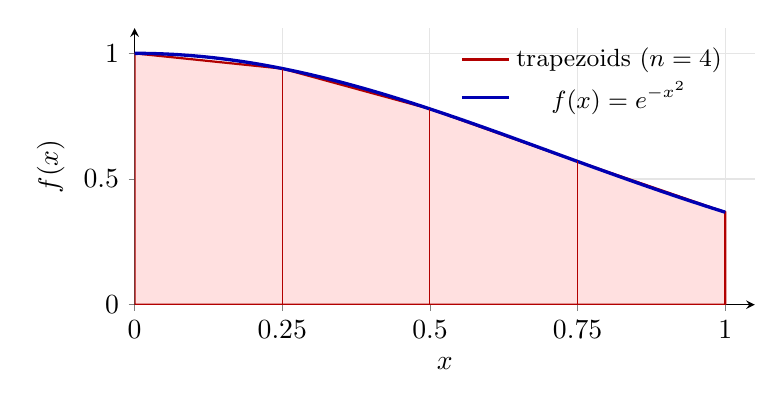
\begin{tikzpicture}
    \begin{axis}[
        width=0.78\textwidth, height=0.42\textwidth,
        xlabel={$x$}, ylabel={$f(x)$},
        xmin=0, xmax=1.05, ymin=0, ymax=1.1,
        xtick={0,0.25,0.5,0.75,1}, ytick={0,0.5,1},
        axis lines=left, grid=both, grid style={gray!20},
        legend style={at={(0.97,0.97)},anchor=north east,font=\small,draw=none,fill=none},
      ]
      \addplot[red!70!black,thick,fill=red!12] coordinates
        {(0,0) (0,1) (0.25,0.939413) (0.5,0.778801) (0.75,0.569783) (1,0.367879) (1,0)} \closedcycle;
      \addlegendentry{trapezoids ($n=4$)}
      \addplot[blue!70!black,very thick,domain=0:1,samples=100] {exp(-x^2)};
      \addlegendentry{$f(x)=e^{-x^{2}}$}
      \foreach \xx in {0.25,0.5,0.75}{
        \addplot[red!70!black,thin] coordinates {(\xx,0) (\xx,{exp(-\xx^2)})};
      }
    \end{axis}
  \end{tikzpicture}
  \caption{The function $f(x)=e^{-x^{2}}$ on $[0,1]$ and the four trapezoids of the rule $T_4$.}
  \label{fig:trap}
\end{figure}

\begin{table}[htbp]
  \centering
  \caption{Approximations and absolute errors for $\int_0^1 e^{-x^2}\,\mathrm{d}x$.}
  \label{tab:results}
  \sisetup{table-format=1.6,round-mode=none}
  \begin{tabular}{r S S S[table-format=1.3e-2] S[table-format=1.3e-2]}
    \toprule
    {$n$} & {$T_n$} & {$S_n$} & {$\lvert I-T_n\rvert$} & {$\lvert I-S_n\rvert$} \\
    \midrule
     2 & 0.731370 & 0.747180 & 1.545e-2 & 3.563e-4 \\
     4 & 0.742984 & 0.746855 & 3.840e-3 & 3.125e-5 \\
     8 & 0.745866 & 0.746826 & 9.585e-4 & 1.988e-6 \\
    16 & 0.746585 & 0.746824 & 2.395e-4 & 1.246e-7 \\
    \bottomrule
  \end{tabular}
\end{table}

\section{Conclusion}
Simpson's rule is much more accurate than the trapezoidal rule for this smooth integrand.
When $n$ is doubled, the error of the trapezoidal rule is divided by about $4$ (order $h^{2}$), whereas the error of Simpson's rule is divided by about $16$ (order $h^{4}$), in agreement with \cref{eq:trap-err,eq:simpson-err}.
For further reading, see~\cite{burden2016,atkinson1989,press2007}.

\printbibliography

\end{document}


